
\iffalse \bibliography{../bibliography.bib} \fi

\chapter{Results} \label{results}

\section{Images}

The following screenshots were rendered at around 180 frames per second with a 2560x1440 resolution.
The test machine was a desktop computer with an Intel i7-5820K 3.3GHz CPU, a Nvidia GTX 980 GPU, and 16 GB of RAM.

Figures \ref{fig:screenshot00} and \ref{fig:screenshot01} show a view of a forest region with mountain regions in the distance.
Figures \ref{fig:screenshot02} and \ref{fig:screenshot03} show a mountain region.
Figure \ref{fig:screenshot04} shows the same view of the previous mountain screenshot with a different sun position.
Figure \ref{fig:screenshot05} shows a lake and figure \ref{fig:screenshot06} shows a shore cliff.

\begin{figure}
	\centering
		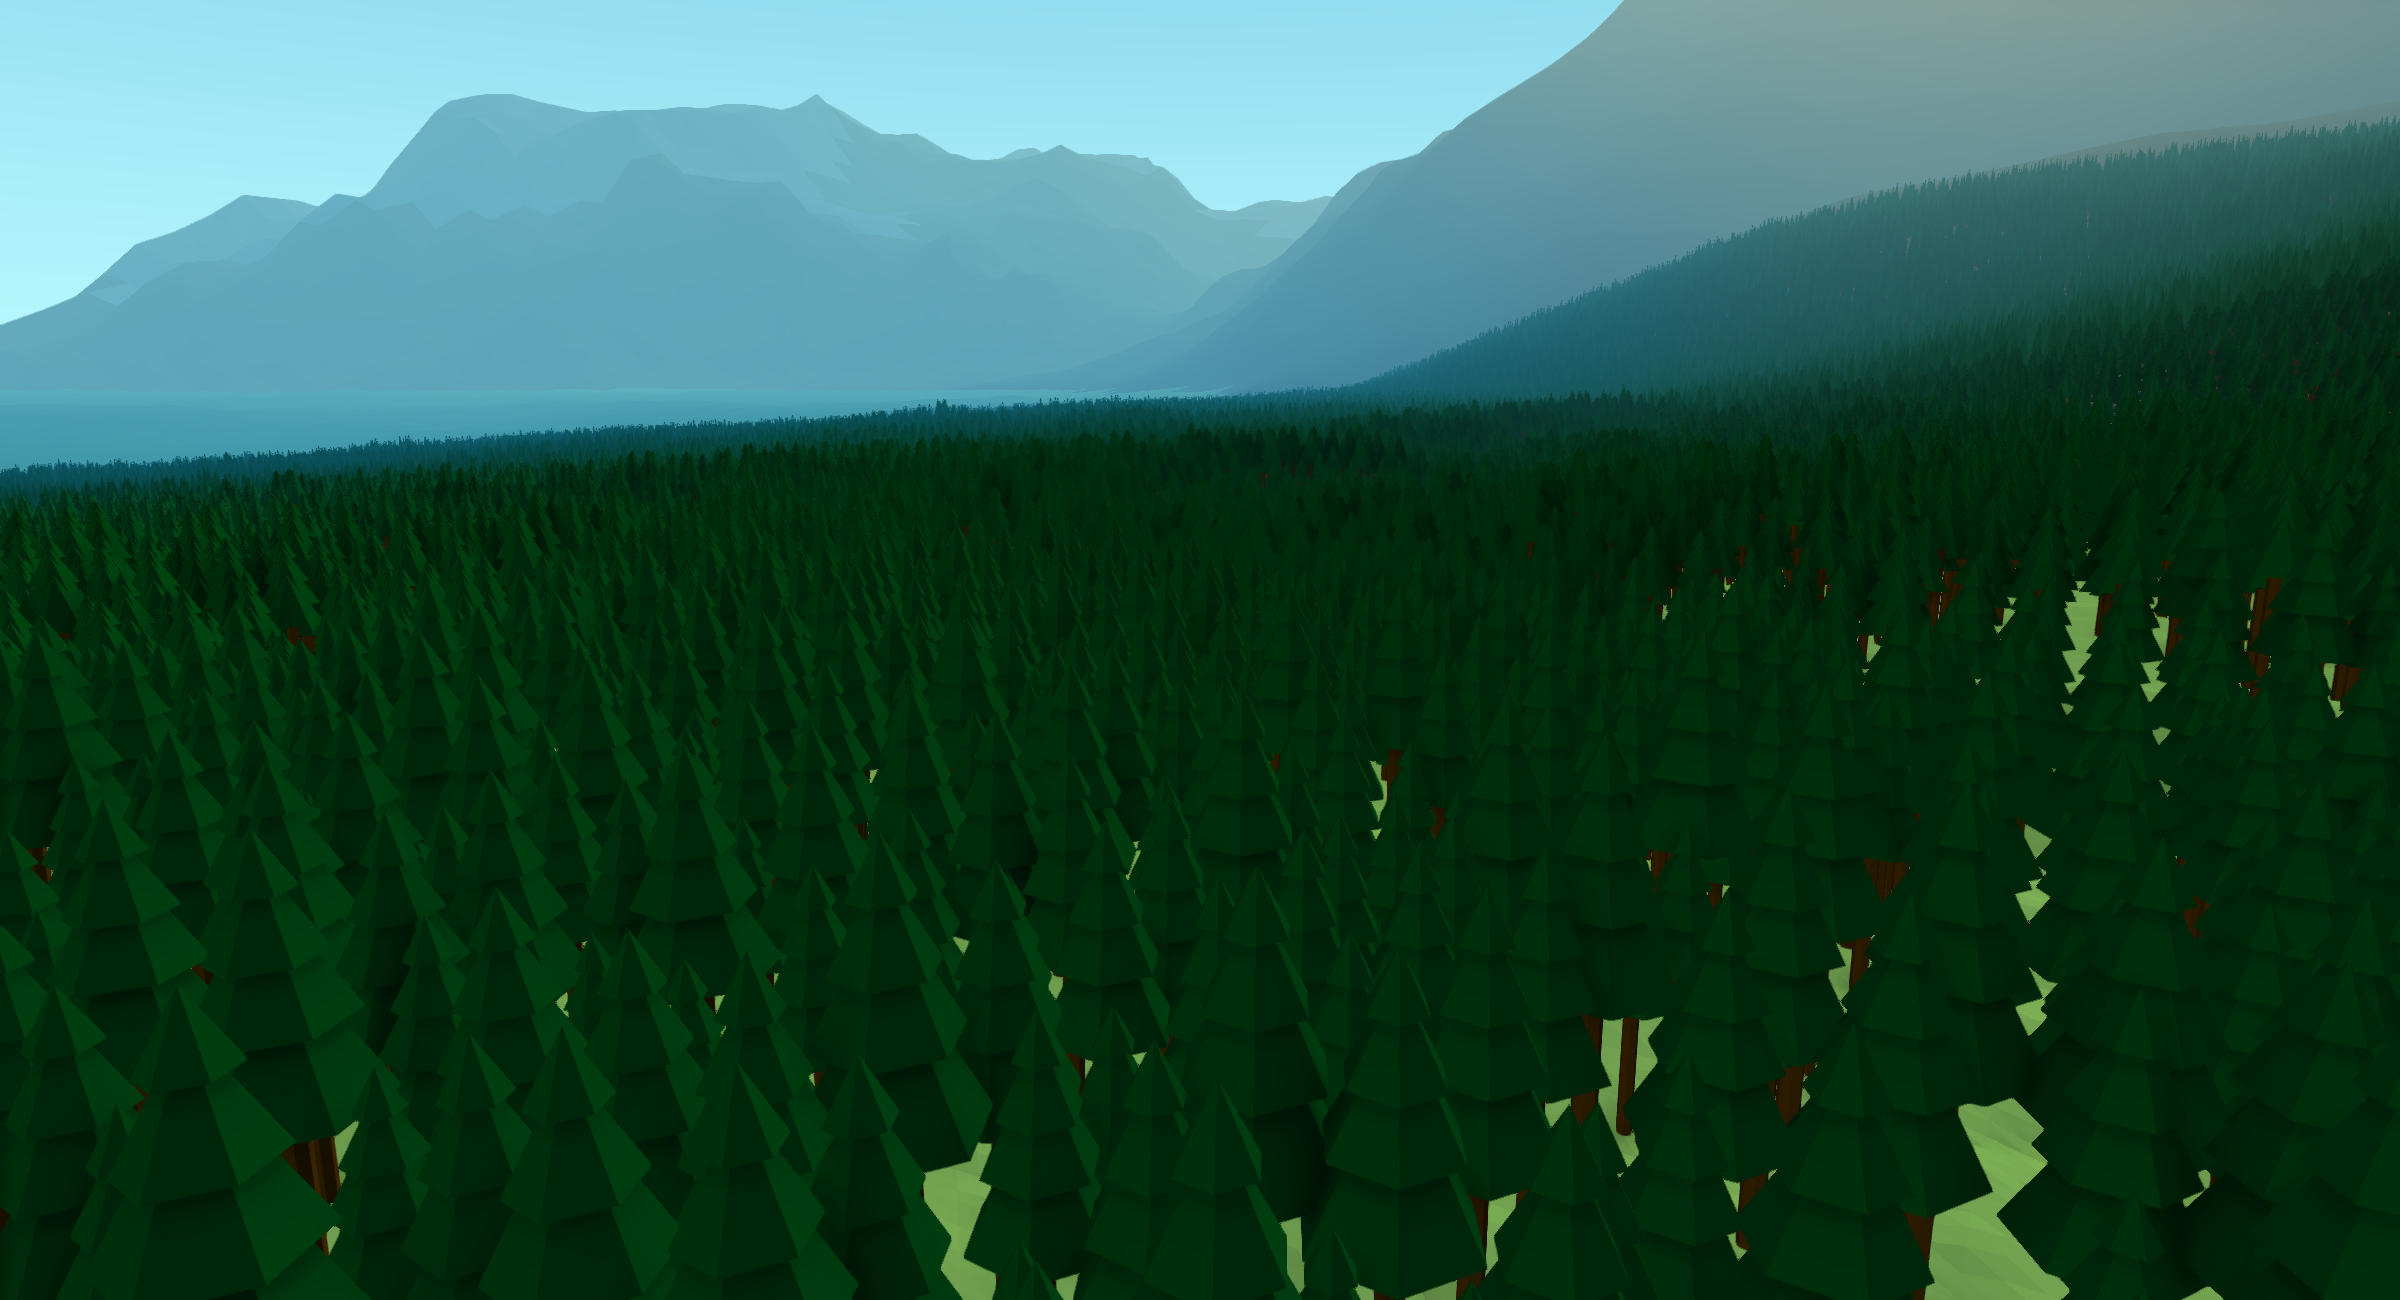
\includegraphics[width=1.0\textwidth]{figures/Screenshot000000.png}
	\caption{Forest region.}
	\label{fig:screenshot00}
\end{figure}

\begin{figure}
	\centering
		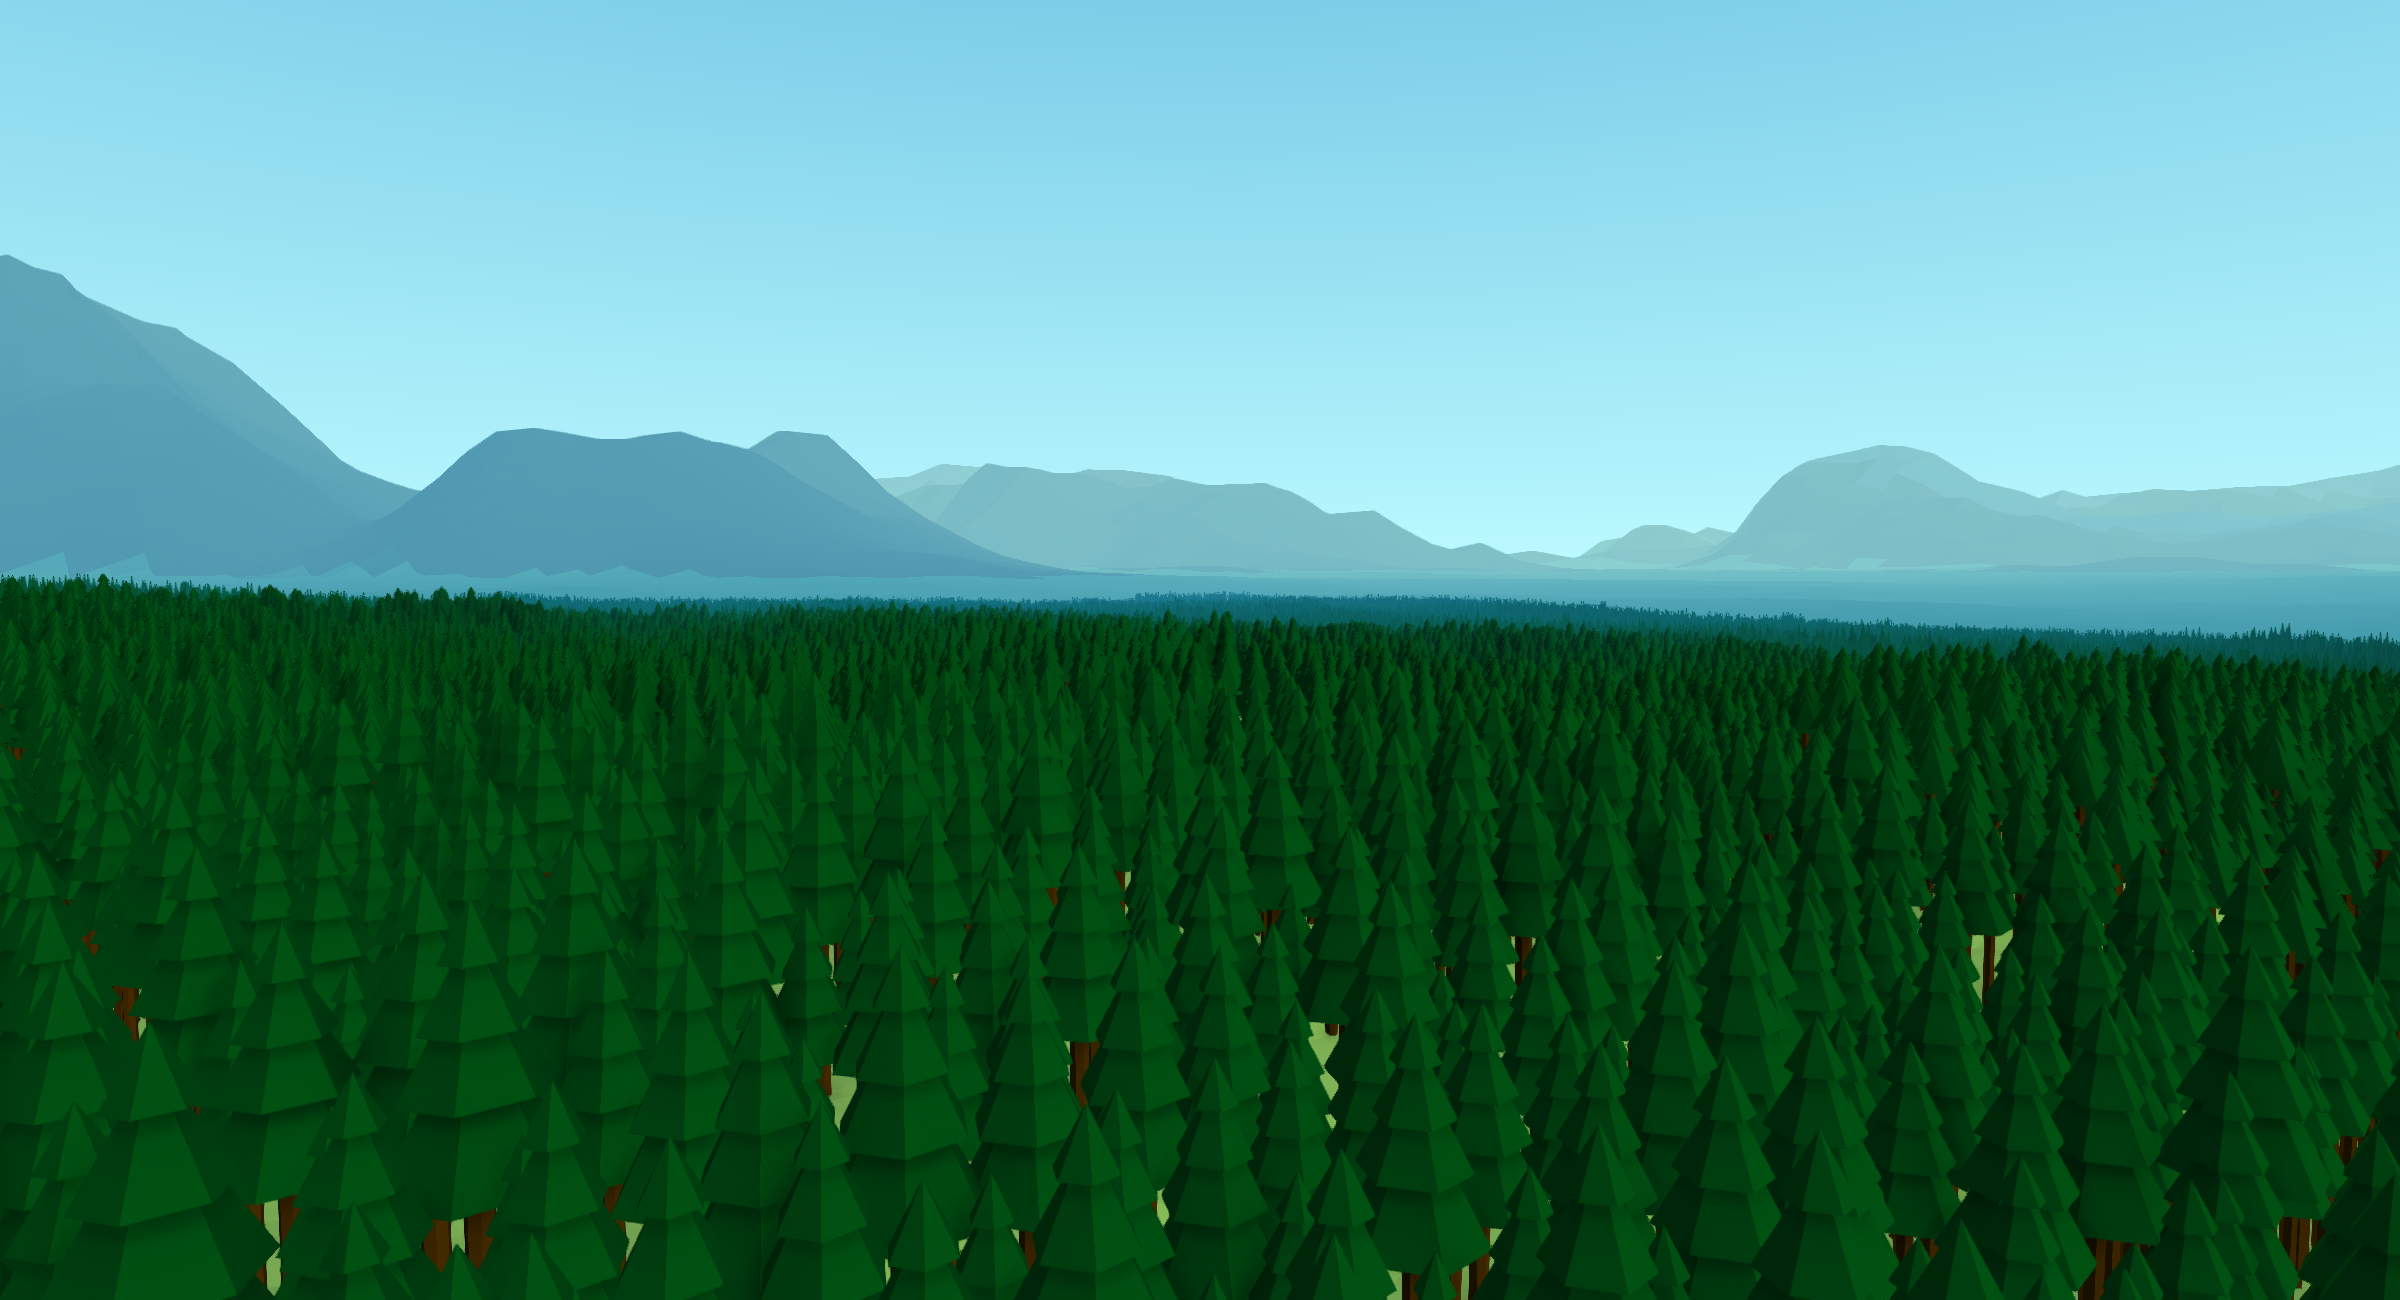
\includegraphics[width=1.0\textwidth]{figures/Screenshot000001.png}
	\caption{Another view of a forest region.}
	\label{fig:screenshot01}
\end{figure}

\begin{figure}
	\centering
		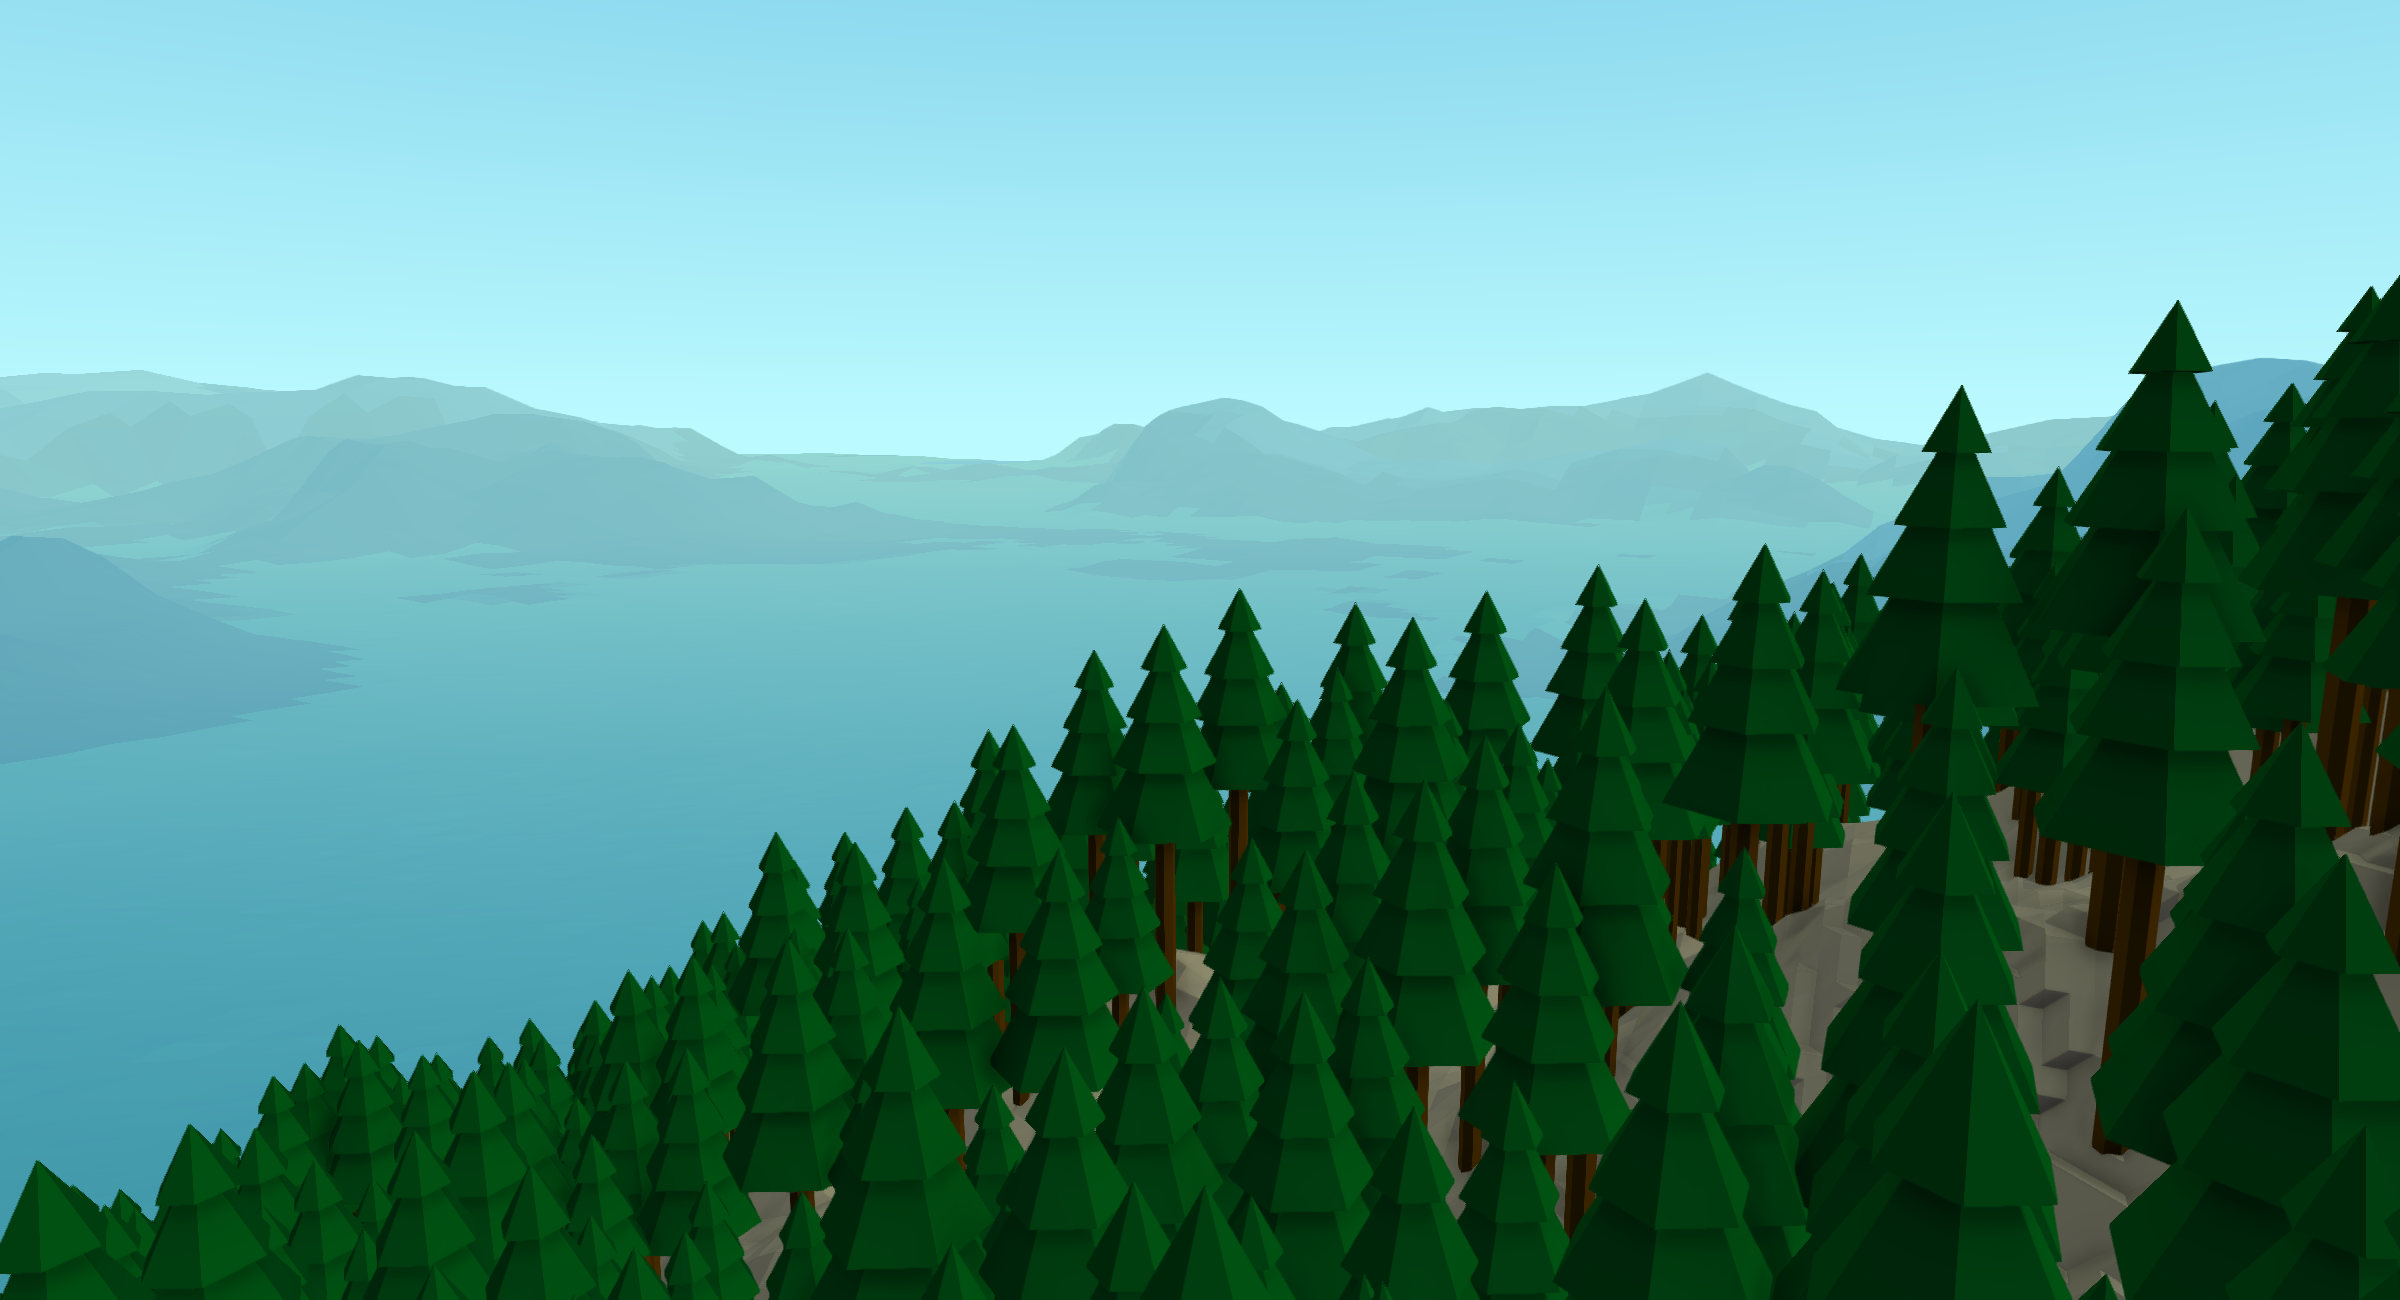
\includegraphics[width=1.0\textwidth]{figures/Screenshot000002.png}
	\caption{Mountain region.}
	\label{fig:screenshot02}
\end{figure}

\begin{figure}
	\centering
		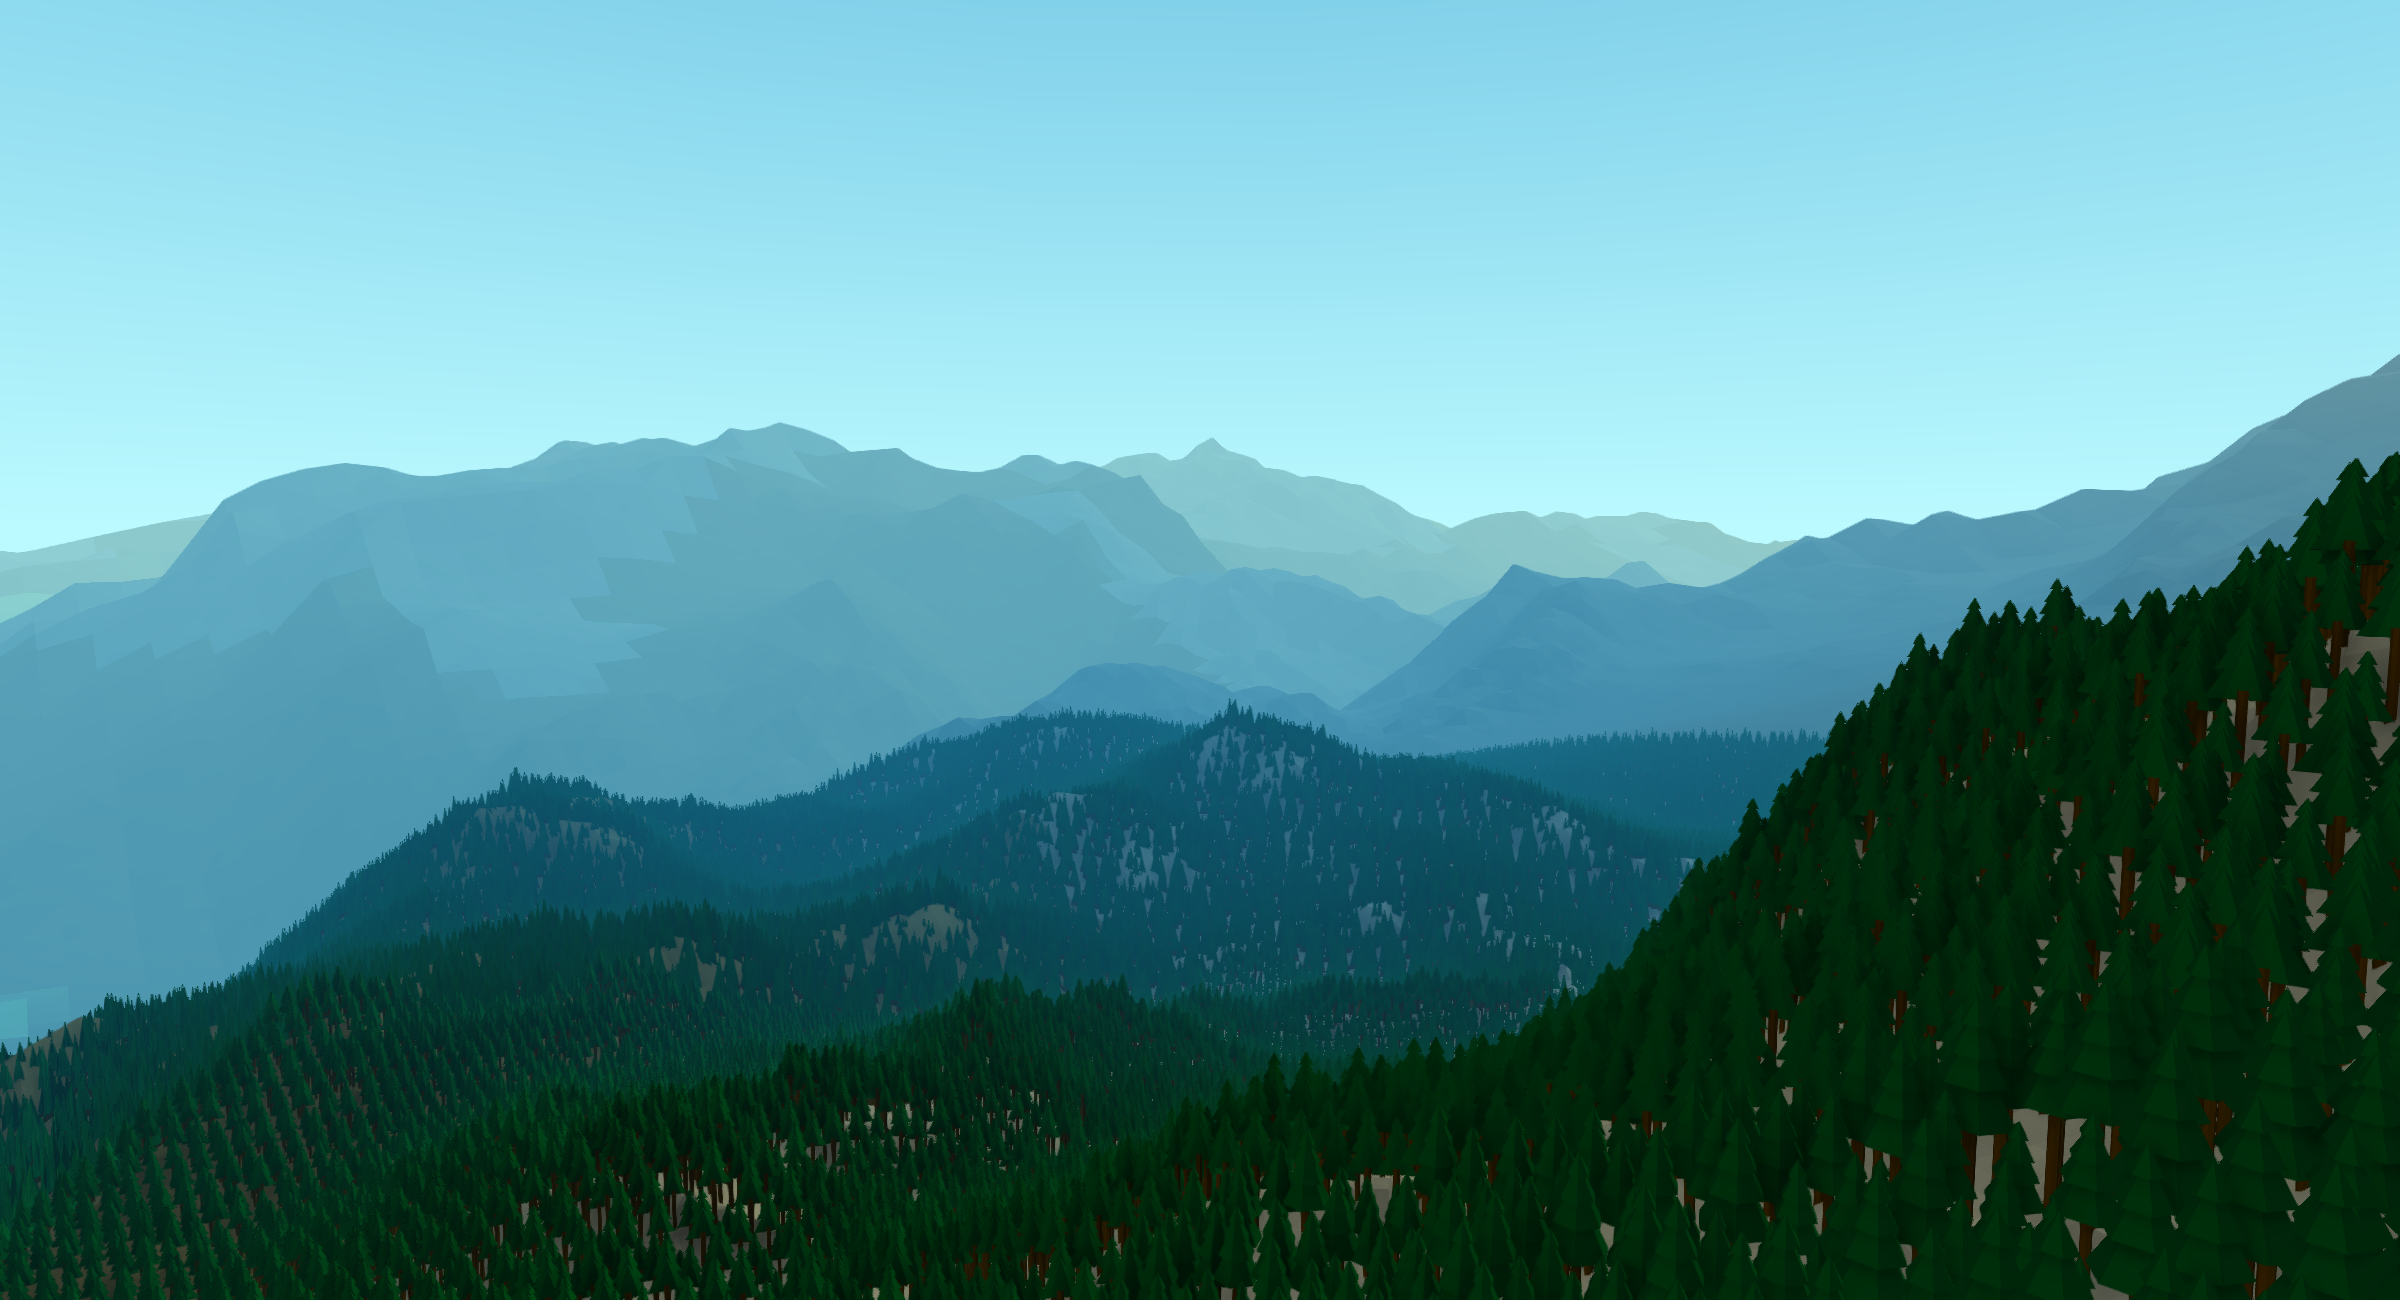
\includegraphics[width=1.0\textwidth]{figures/Screenshot000003.png}
	\caption{Mountain region with distant trees.}
	\label{fig:screenshot03}
\end{figure}

\begin{figure}
	\centering
		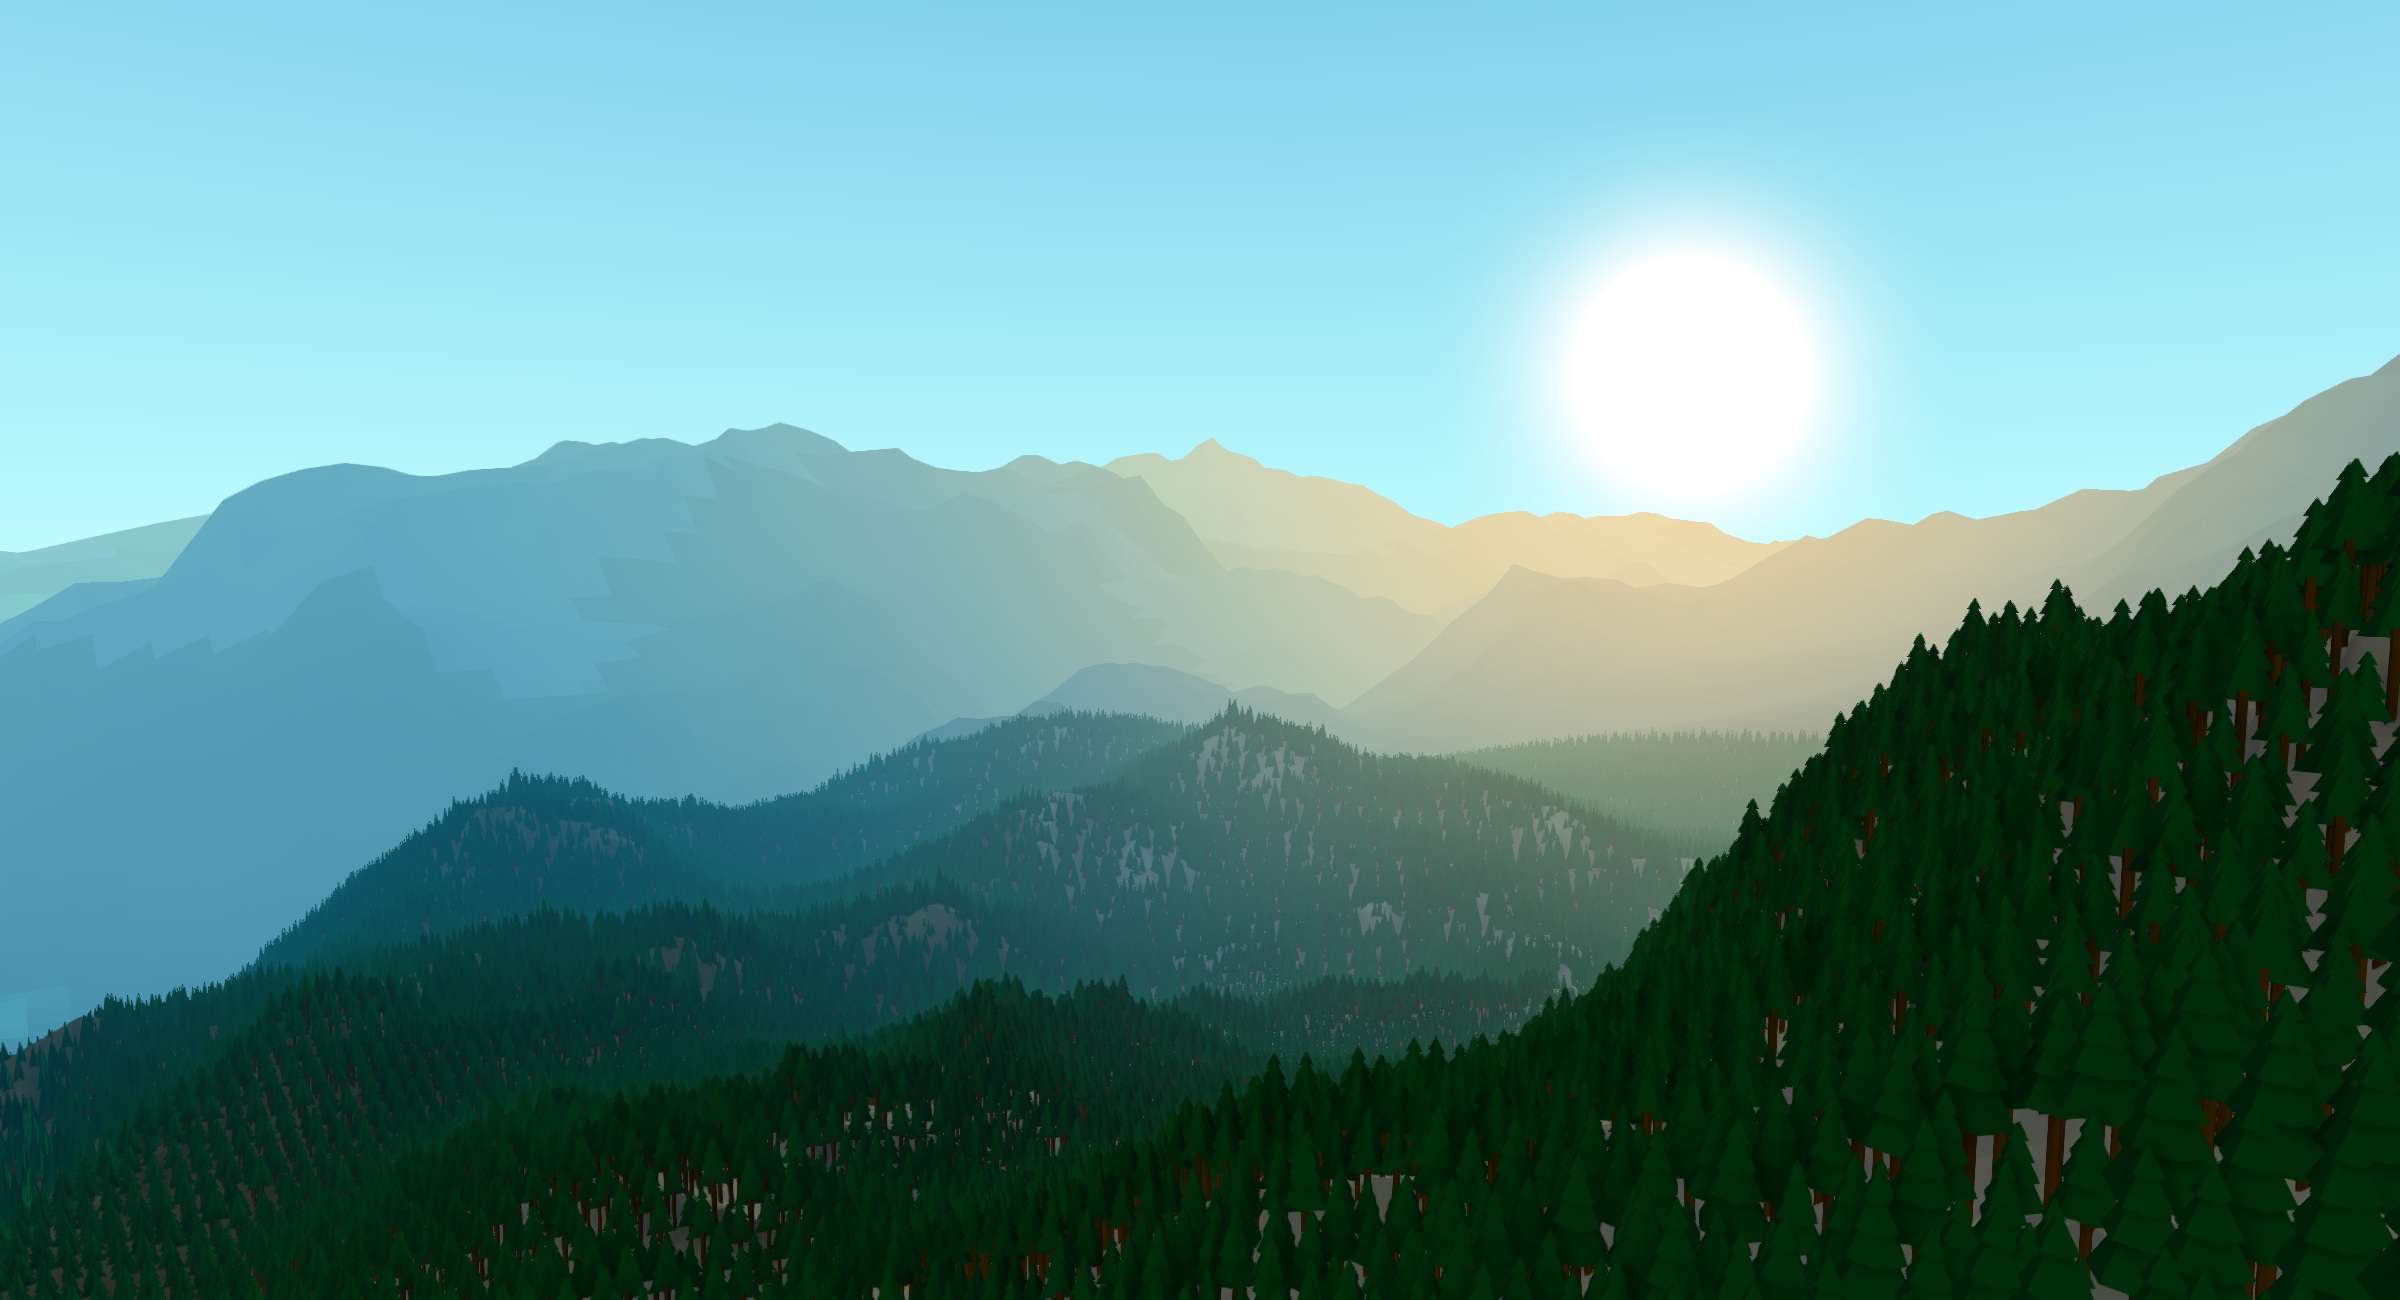
\includegraphics[width=1.0\textwidth]{figures/Screenshot000004.png}
	\caption{Same view as the previous screenshot, with different sun position.}
	\label{fig:screenshot04}
\end{figure}

\begin{figure}
	\centering
		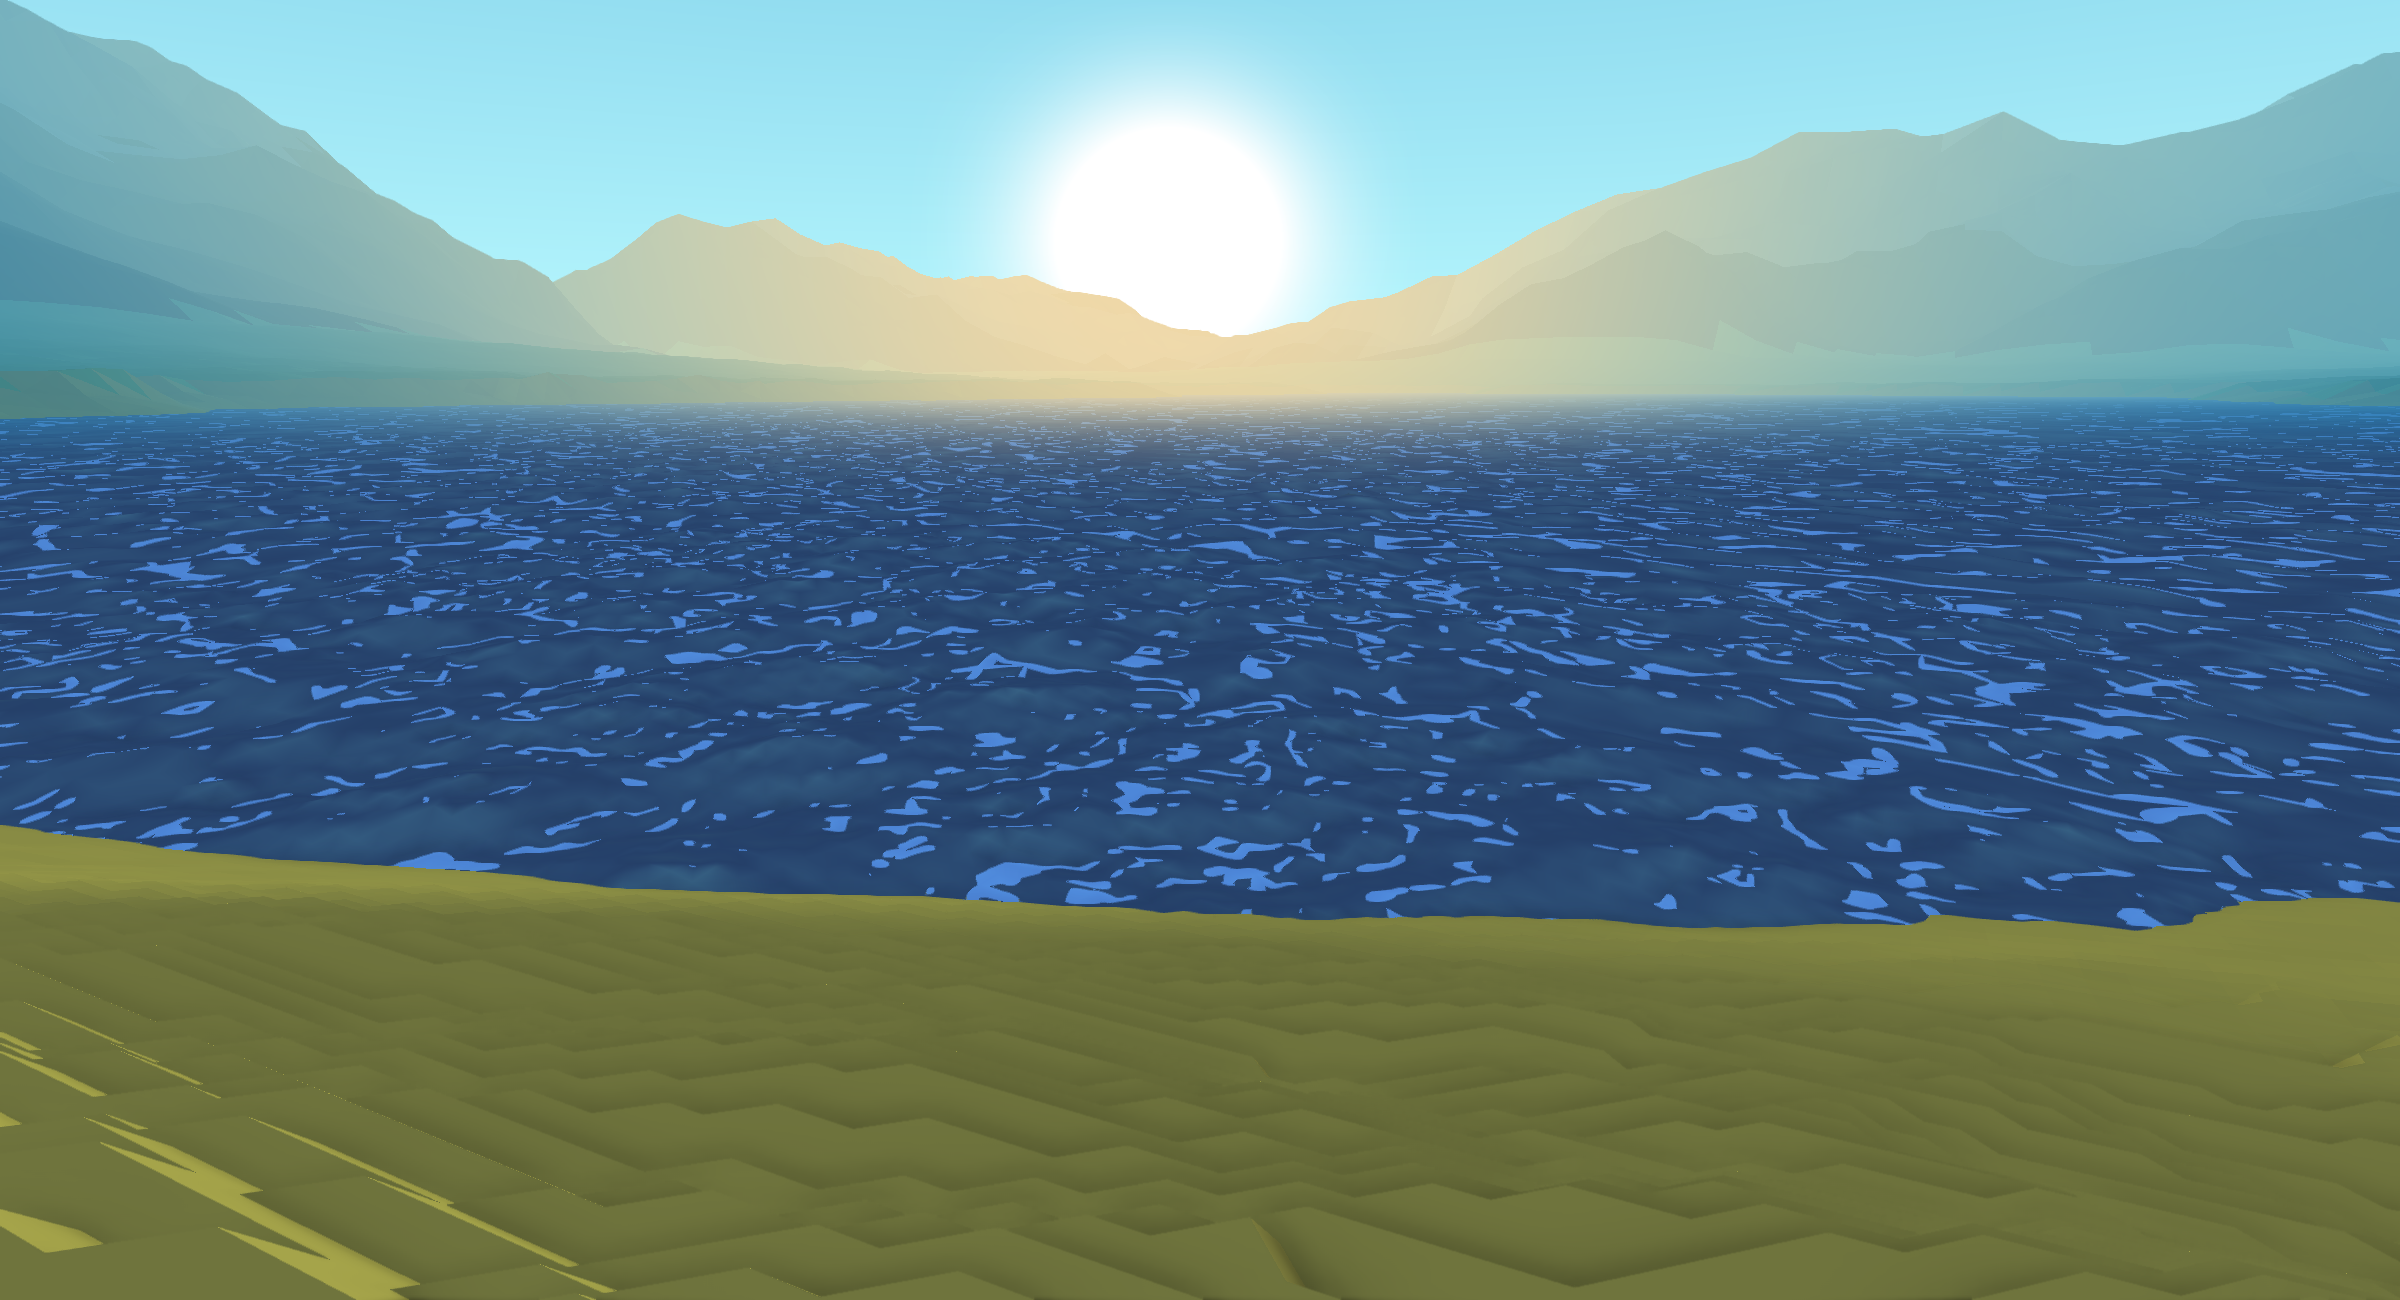
\includegraphics[width=1.0\textwidth]{figures/Screenshot000005.png}
	\caption{A lake.}
	\label{fig:screenshot05}
\end{figure}

\begin{figure}
	\centering
		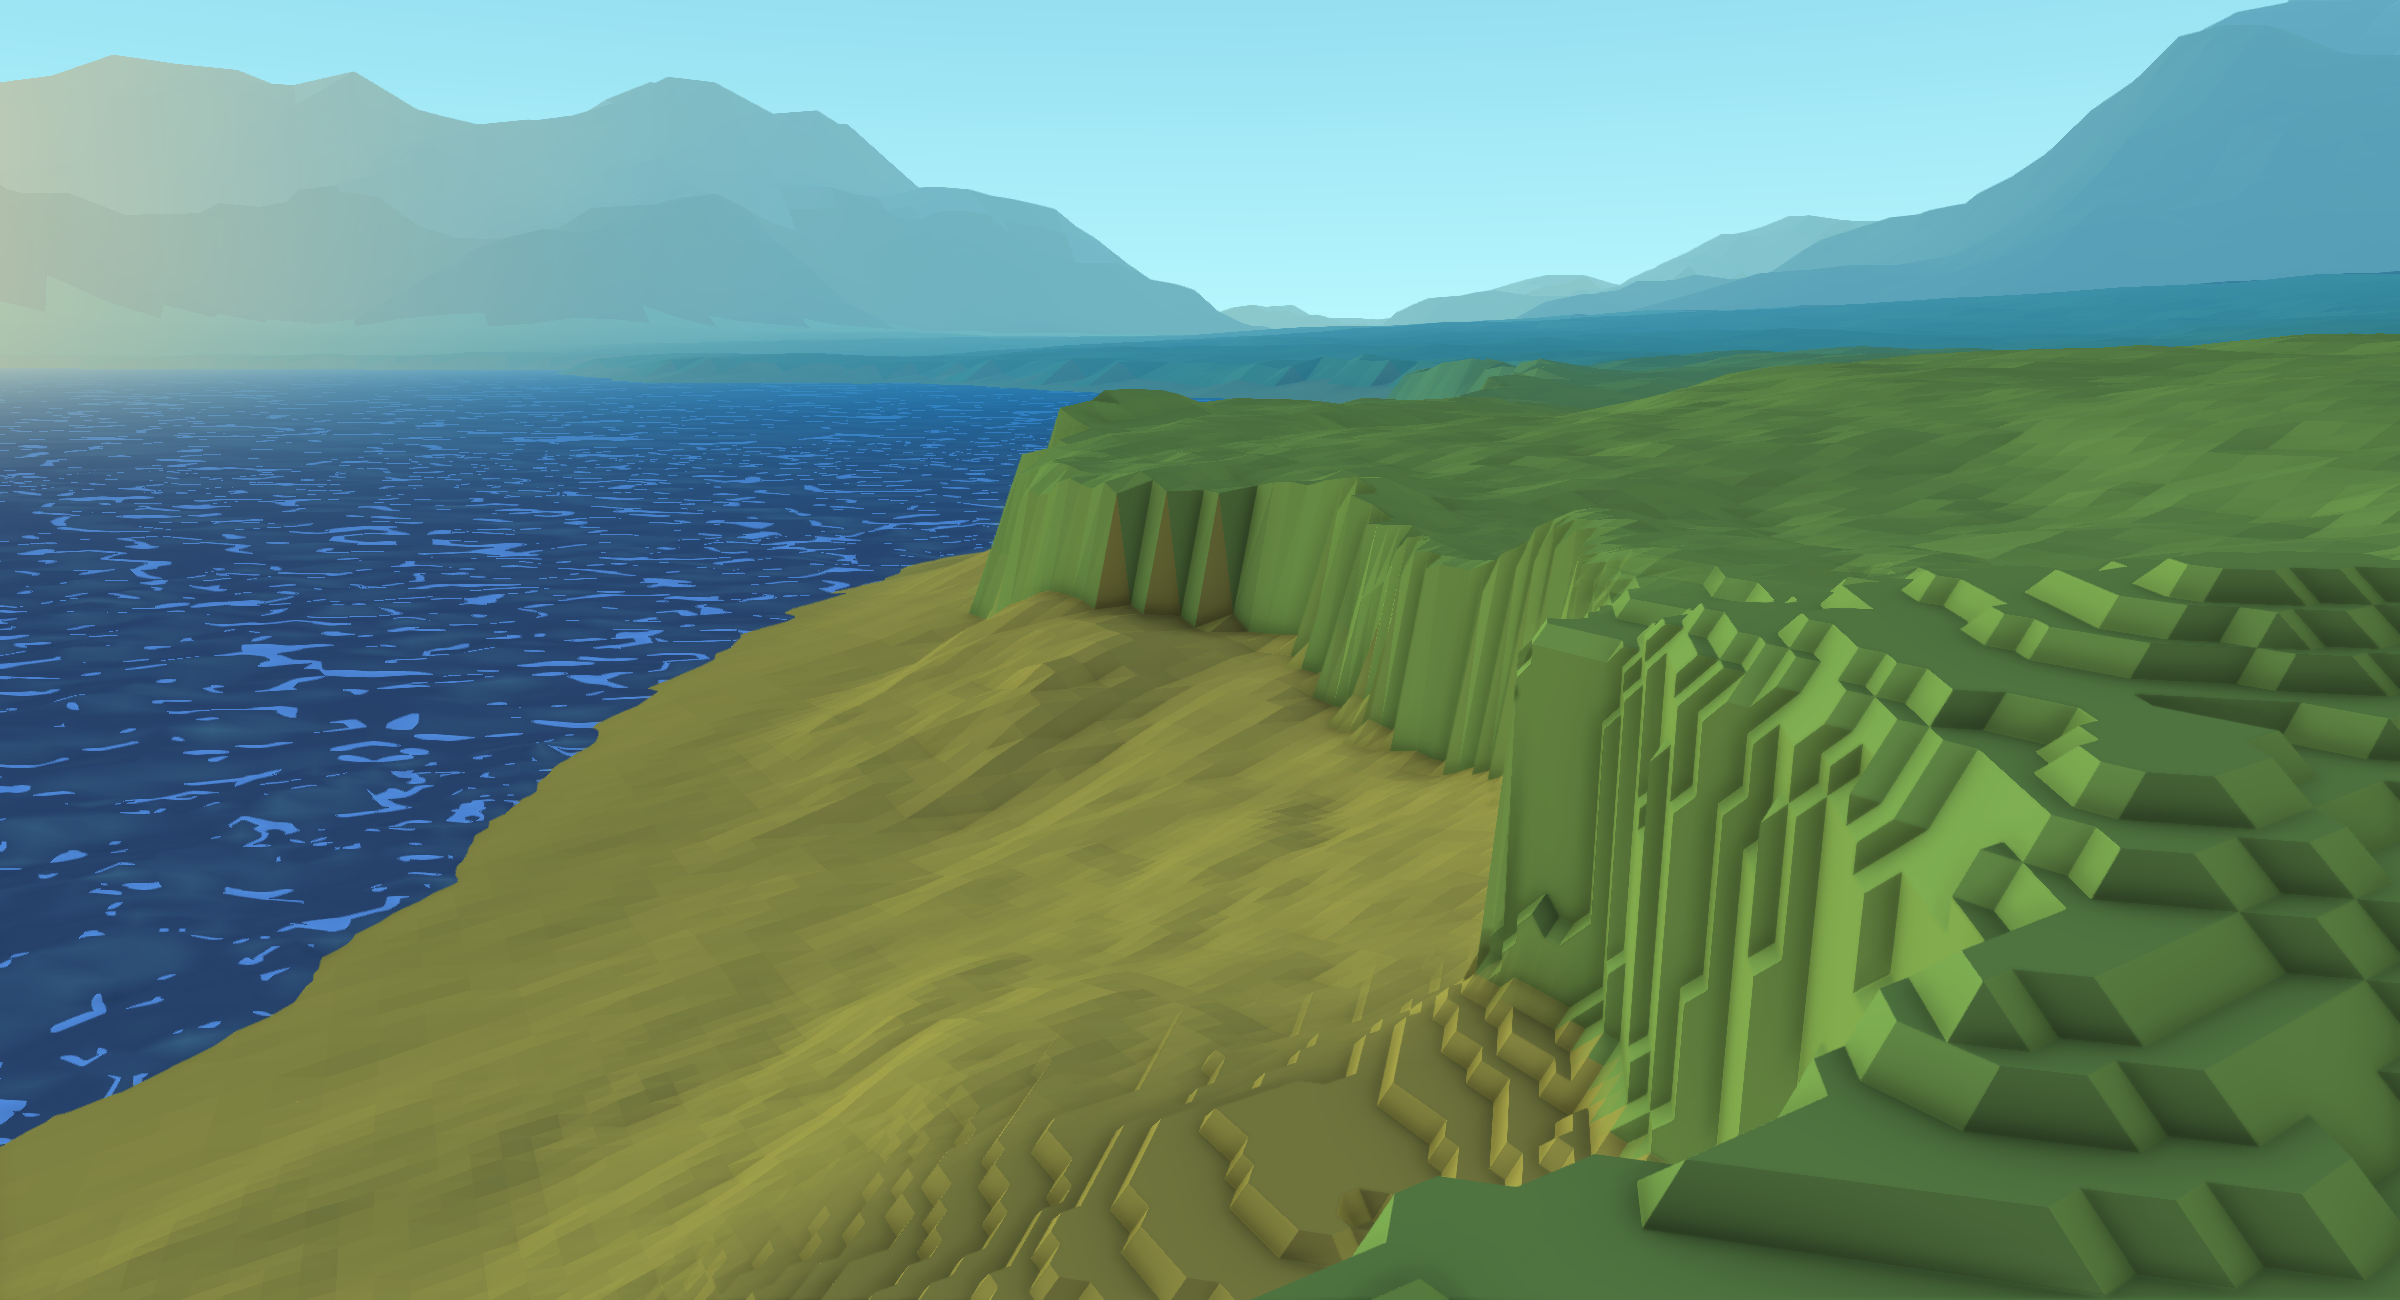
\includegraphics[width=1.0\textwidth]{figures/Screenshot000006.png}
	\caption{Shoreline cliff.}
	\label{fig:screenshot06}
\end{figure}

\section{Voxels}

The size of voxel chunks affects rendering performance and the cost of modification.
Since modifying the terrain requires the entire chunk mesh to be reconstructed, it is ideal to have smaller chunks.
However, larger chunk sizes reduce the number of draw calls.
Figure \ref{fig:voxel_plot_1} shows the relationship between chunk size and render performance for a fixed view distance.
Since the same amount of geometry is rendered for each chunk size tested, the decrease in performance at low chunk size can be attributed to draw calls and other engine overhead.
Figure \ref{fig:voxel_plot_2} shows the modification cost for each chunk size.
These results indicate that that a chunk size of 32 or 64 is a good compromise between render performance and modification cost.

\begin{figure}
	\centering
\begin{tikzpicture}
	\begin{axis}[
		xlabel=Chunk Size (ft),
		ylabel=Frame Time (ms),
		width=11cm
		]
		\addplot[color=green,mark=*] coordinates
		{
			(4,649.37)
			(8,163.43)
			(16,40.69)
			(32,9.04)
			(64,2.27)
			(128,2.16)
			(256,1.85)
		};
	\end{axis}
\end{tikzpicture}
	\caption{
		Voxel terrain rendering performance for different chunk sizes.
		For each chunk size, view distance is set to 512 feet.
	}
	\label{fig:voxel_plot_1}
\end{figure}

\begin{figure}
	\centering
\begin{tikzpicture}
	\begin{axis}[
		xlabel=Chunk Size (ft),
		ylabel=Modification Time (s),
		width=11cm
		]
		\addplot[color=green,mark=*] coordinates
		{
			(4,0.0002)
			(8,0.0010)
			(16,0.0068)
			(32,0.0342)
			(64,0.301)
			(128,2.42)
			(256,24.44)
		};
	\end{axis}
\end{tikzpicture}
	\caption{
		Graph of modification cost (i.e. digging) for different chunk sizes.
	}
	\label{fig:voxel_plot_2}
\end{figure}

\section{Clipmaps}

One major motivation for using geometry clipmaps  is the exponential relationship between layer count and view distance.
Figures \ref{fig:clipmaps_plot_1} and \ref{fig:clipmaps_plot_2} show the relationship between clipmap layers, view distance, and frame time in milliseconds for a scene containing only the clipmaps terrain and a skybox.

\begin{figure}
	\centering
\begin{tikzpicture}
	\begin{axis}[
		xlabel=Layer Count,
		ylabel=Frame Time (ms),
		width=11cm
		]
		\addplot[color=red,mark=*] coordinates
		{
			(1,0.245)
			(2,0.27)
			(3,0.28)
			(4,0.288)
			(5,0.305)
			(6,0.321)
			(7,0.342)
			(8,0.351)
			(9,0.37)
			(10,0.389)
			(11,0.412)
			(12,0.435)
			(13,0.442)
			(14,0.447)
			(15,0.453)
			(16,0.463)
			(17,0.476)
			(18,0.485)
		};
	\end{axis}
\end{tikzpicture}
	\caption{
		Geometry clipmaps render time for a given number of clipmap layers.
		Note that the frame-time is always sub-millisecond, even for a large number of layers.
	}
	\label{fig:clipmaps_plot_1}
\end{figure}

\begin{figure}
	\centering
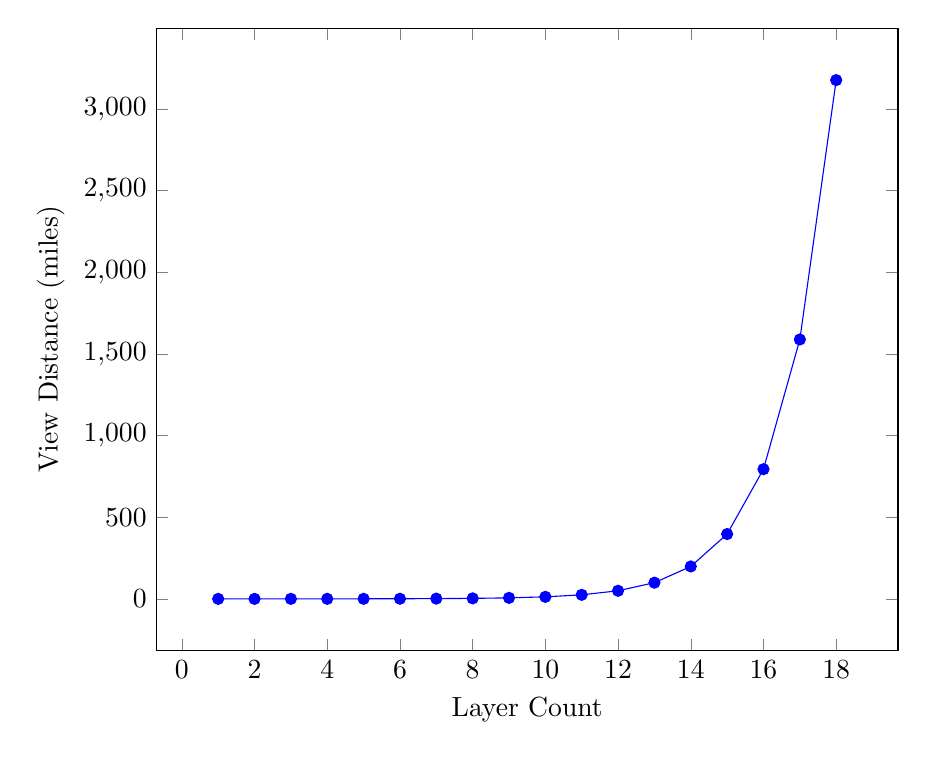
\begin{tikzpicture}
	\begin{axis}[
		xlabel=Layer Count,
		ylabel=View Distance (miles),
		width=11cm
		]
		\addplot[color=blue,mark=*] coordinates
		{
			(1,0.024242424)
			(2,0.048484848)
			(3,0.096969697)
			(4,0.193939394)
			(5,0.387878788)
			(6,0.775757576)
			(7,1.551515152)
			(8,3.103030303)
			(9,6.206060606)
			(10,12.41212121)
			(11,24.82424242)
			(12,49.64848485)
			(13,99.2969697)
			(14,198.5939394)
			(15,397.1878788)
			(16,794.3757576)
			(17,1588.751515)
			(18,3177.50303)
		};
	\end{axis}
\end{tikzpicture}
	\caption{
		Geometry clipmaps view distance and for a given number of clipmap layers.
	}
	\label{fig:clipmaps_plot_2}
\end{figure}

There is a linear relationship between frame time and layer count, but an exponential relationship between view distance and layer count.
For a relatively minor increase in frame time an absurd view distance of over 3000 miles can be achieved.
For reference, the largest possible view distance on earth is around 300 miles, between two mountains in South America. \cite{viewdistancemaxearth}

Larger individual layer sizes increase view distance and reduce polygon screen-space at the cost of performance.
The addition of a geometry shader normal calculation simplifies the terrain generation process and improves visual quality, but incurs a small performance hit.
We found a frame time increase of about 0.01 ms when using 11 layers.


\section{Vegetation}

The far layers of the vegetation system are rough visual approximations of the closeup tree meshes, but are significantly less costly for rendering.
Figure \ref{fig:tree_plot_1} shows the cost of rendering a large number of each type of representation.

Increasing the size of tree groups improves rendering performance by reducing the number of draw calls, but also causes larger CPU lag spikes when a new group of trees has to be generated.
Figure \ref{fig:tree_plot_2} shows the render performance for each group size.

\begin{figure}
	\centering
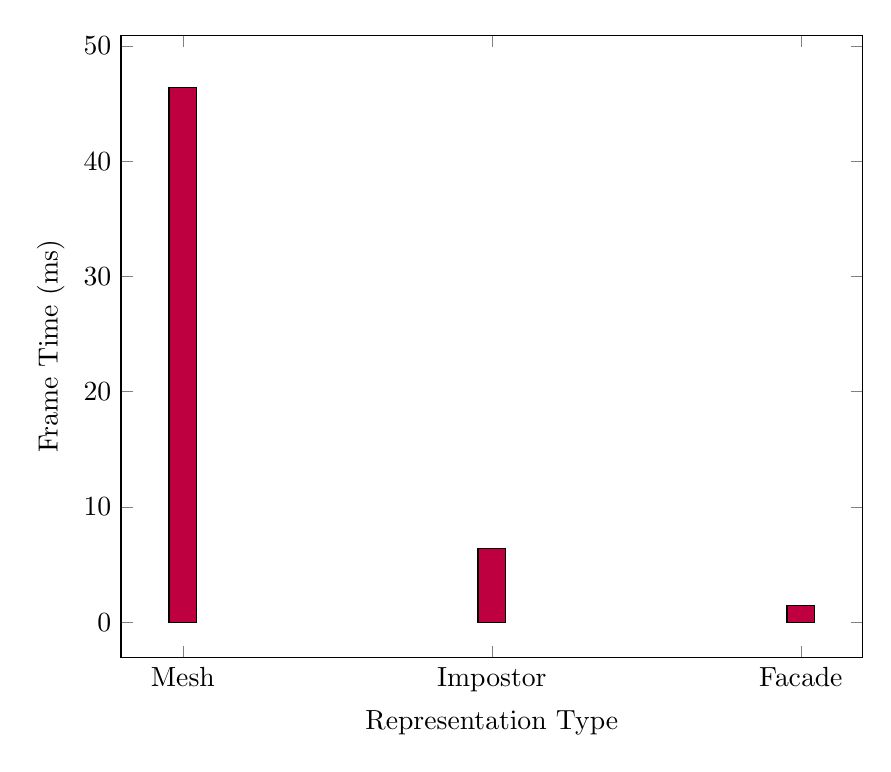
\begin{tikzpicture}
	\begin{axis}[
		symbolic x coords={Mesh, Impostor, Facade},
		xtick=data,
		xlabel=Representation Type,
		ylabel=Frame Time (ms),
		width=11cm
		]
		\addplot[ybar,fill=purple] coordinates
		{
			(Mesh, 46.42)
			(Impostor, 6.38)
			(Facade, 1.42)
		};
	\end{axis}
\end{tikzpicture}
	\caption{
		Tree performance vs. tree representation type, view distance set to 1280 feet.
	}
	\label{fig:tree_plot_1}
\end{figure}

\begin{figure}
	\centering
\begin{tikzpicture}
	\begin{axis}[
		xlabel=Group Size (ft),
		ylabel=Frame Time (ms),
		width=11cm,
		ymin=0
		]
		\addplot[color=orange,mark=*] coordinates
		{
			(40, 20.48)
			(80, 5.46)
			(160, 2.90)
			(320, 2.56)
		};
	\end{axis}
\end{tikzpicture}
	\caption{
		Tree performance vs. tree group size.
	}
	\label{fig:tree_plot_2}
\end{figure}
